%!TEX root = jir2018aspects.tex
\subsection{Information Foraging Theory} \label{sec:ift}

%As previously mentioned, in ad hoc topic retrieval the user is tasked with finding a number of relevant documents about a particular topic. The main focus in ad hoc topic retrieval is on whether documents are relevant or not, and not whether they are different. Whereas, in aspectual retrieval task, documents have to satisfy both conditions. For example, lets say the topic is ``wildlife extinction'', where the searcher needs to write a report based on examples. In the ad hoc task, if the user finds several documents regarding ``Pandas in China'' then these would be considered relevant. In the aspectual retrieval task, where the search needs to write a report based on a number of different examples/species, then the first document found regarding ``Pandas in China'' is considered relevant/useful, and other aspects (in this case species) would need to be found, e.g. ``Sumatran Rhinos in Malaysia'', ``Ibis in Japan'', etc. 

To motivate our hypotheses, we draw upon \emph{Information Foraging Theory (IFT)}~\cite{pirolli1999ift}, and, in particular, the \textit{patch model} (a constituting model of IFT) to ground our research and provide insights into how search behaviours should change. %is of particular relevance here, as 
The patch model predicts how long foragers will stay in a given \emph{patch} before moving to a new patch. Under this model, the analogy with an information seeker is as follows. Moving between patches is like expressing a new query (and thus incurs a moving/querying cost), while staying within a patch is akin to assessing documents. 
%The model also predicts how long a forager should stay in a patch before moving on to the next patch. 
Fig.~\ref{fig_ift_patches} graphically shows the predictions given the theory for two systems (diversified and non-diversified), and the corresponding hypothetical gain curves. In the top left plot (Fig.~\ref{fig_ift_patches} \textbf{(a)}) where a non-diversified system is being used, the gain curve for the ad-hoc retrieval task is higher, as any relevant document contributes to the overall level of gain. However, for the aspectual task, the gain curve is lower. This is because similar relevant documents (discussing an already observed aspect) do not contribute to the overall gain accrued by the searcher.

\begin{figure}[t!]
\begin{center}
        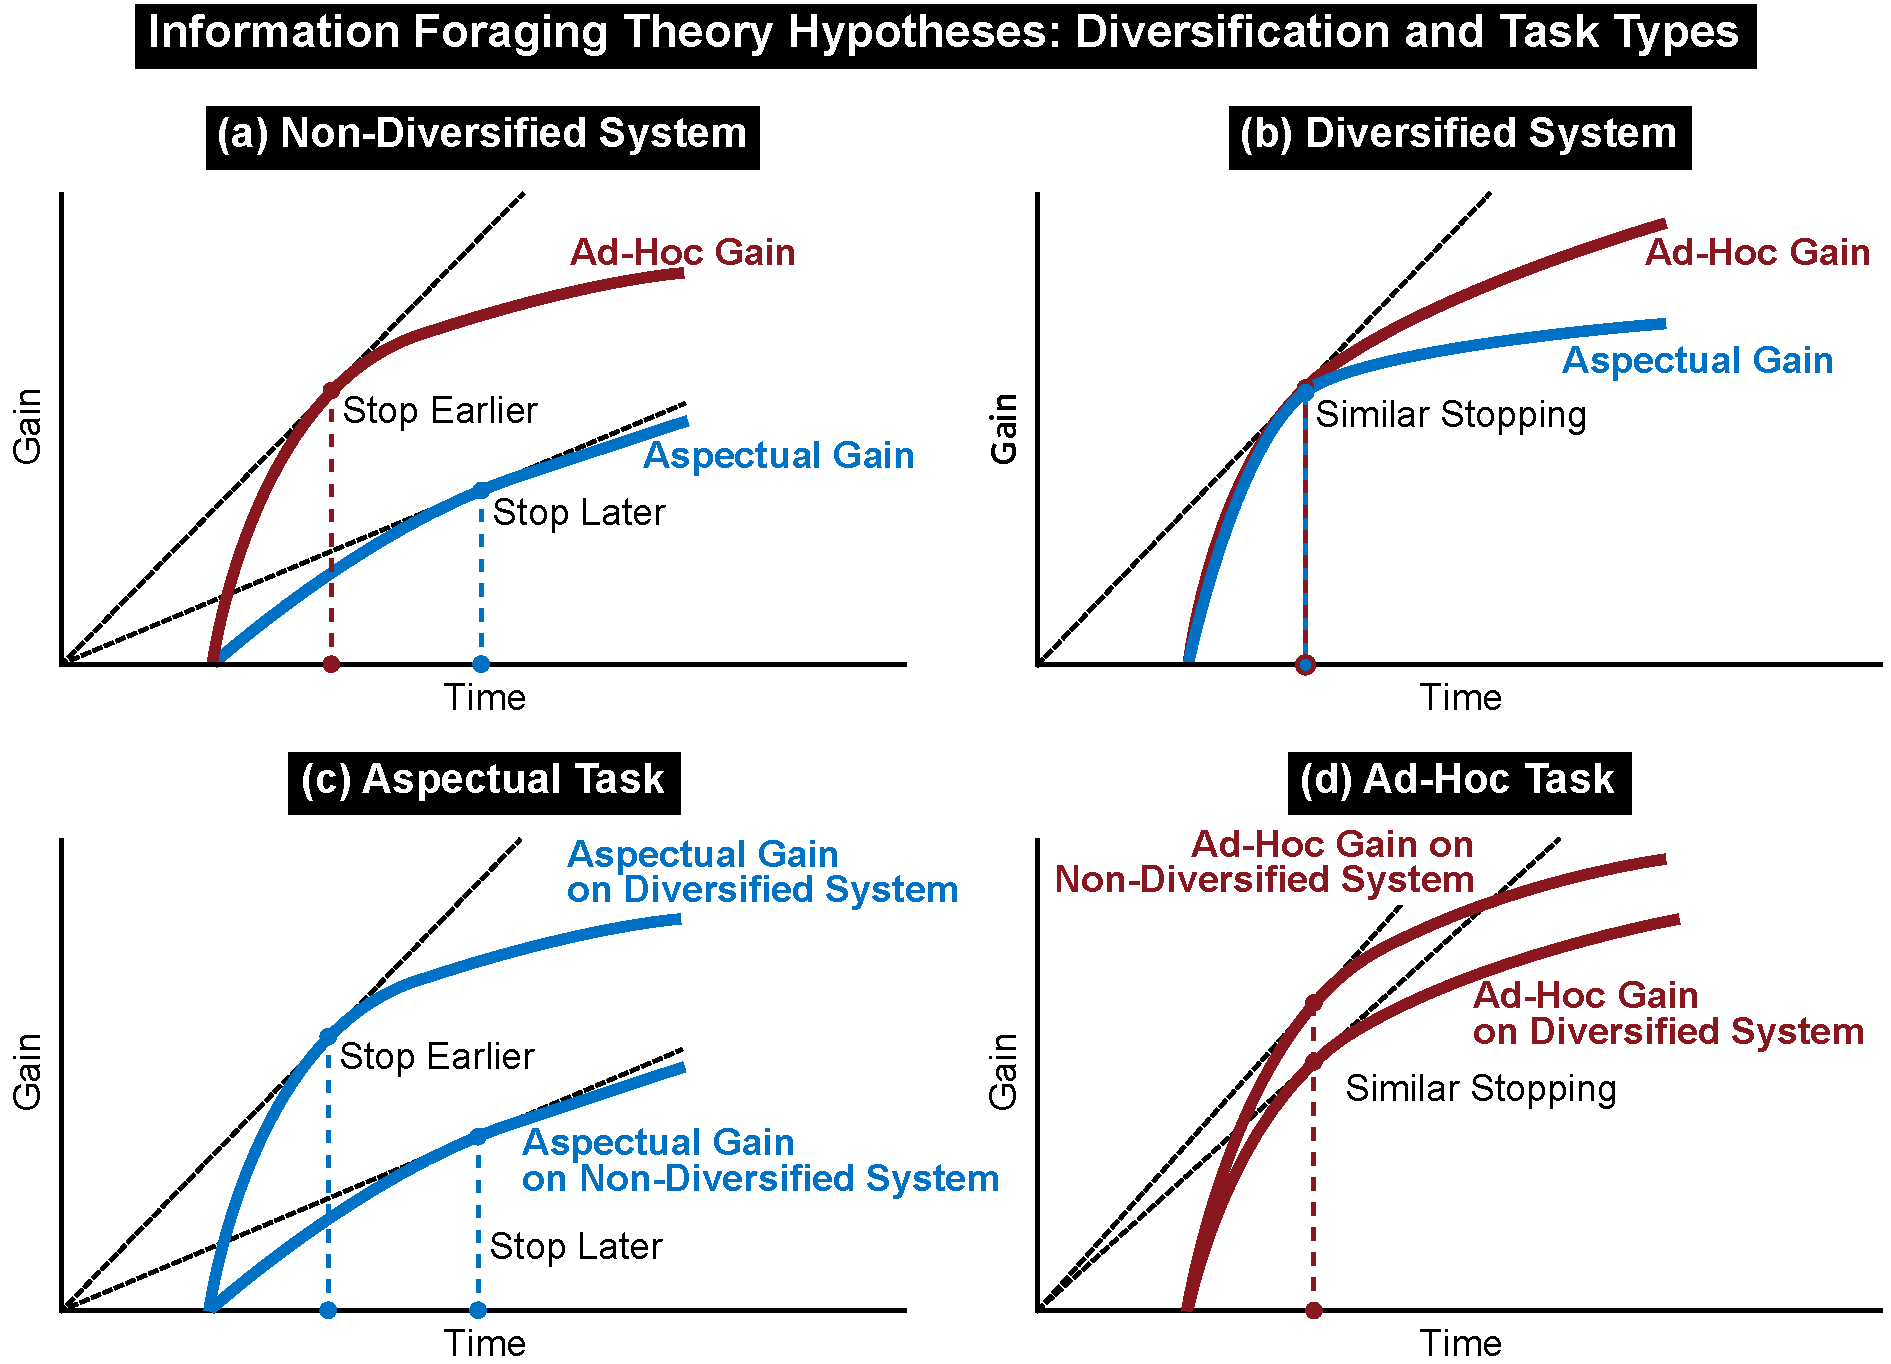
\includegraphics[width=\textwidth]{figures/ift-non-div-fromthesis.pdf}
        \vspace{-2mm}
    \caption{A graphical depiction, using Information Foraging Theory, of how stopping behaviour is likely to be affected with: a system that diversifies results \textbf{(a)}; a system that does not diversify \textbf{(b)}; under an aspectual retrieval task \textbf{(c)}; and under an ad-hoc retrieval task \textbf{(d)}.} \label{fig_ift_patches}    
    \vspace{-6mm}
\end{center}
\end{figure}


From IFT, the optimal stopping point would be different between the two tasks. Graphically, we can find this point by drawing a line from the origin to the tangent of the gain curve -- the red and blue dots indicating the optimal stopping points for ad-hoc and aspectual retrieval, respectively. Thus, IFT suggests that when subjected to the non-diversified system, searchers will examine more documents per query for aspectual retrieval tasks than when compared to ad-hoc retrieval tasks.

In Fig.~\ref{fig_ift_patches} \textbf{(b)} where a diversified system is being used, the gain curves for ad-hoc and aspectual retrieval will be similar. This is because relevant but different documents are discovered earlier. In the case of ad-hoc topic retrieval, these relevant (even if different) documents will still contribute to the overall gain. In the case of aspectual retrieval, the relevant and different documents will also contribute to the searcher's overall gain -- but only up to the point where the documents are similar to the previously retrieved material (i.e. after this point, similar but relevant documents do not contribute to the gain). IFT therefore appears to suggest that similar stopping behaviours would be observed when searchers utilise a system that diversifies results.

Fig.~\ref{fig_ift_patches} \textbf{(c)} shows the predicted stopping behaviour for the aspectual task, where we have plotted the aspectual gain curves from the system plots described above. Interestingly, IFT suggests that searchers will stop sooner when using the diversified system. Therefore, if searching for the same amount of time, searchers would thus issue more queries. Finally, Fig.~\ref{fig_ift_patches} \textbf{(d)} shows the predicted stopping behaviour for ad-hoc retrieval tasks, where again we have plotted the respective gain curves on each system. Note that the gain curve for the the diversifying system may be a little lower as some non-relevant but different material may bubble up the rankings -- but as can be seen, we expect little difference between systems. Therefore, the expected gains and behaviours that we hypothesise will be approximately the same. Consequently, IFT suggests that there will be little difference regarding stopping behaviours between the two systems under ad-hoc retrieval tasks.

In contrast to the hypotheses from IFT, our intuitions suggested that searchers would behave differently such that: when using a standard, non-diversified system, searchers would be more likely to issue a greater number of queries because they would likely need to issue more queries to explore the topic. Indeed, Kelly et al.~\cite{kelly2015search_tasks} showed that more complex search tasks require a greater number of queries to provide sufficient coverage of the topic. For example, if a searcher submits a query such as \texttt{'protecting Pandas in China'} that retrieves relevant material about pandas, we would expect them to only select one or two examples before issuing another query -- rather than examining more results given the current query. In the case of ad-hoc topic retrieval, we would expect that they would issue fewer queries, and examine more documents per query. This is because they don't need to find multiple aspects of the said topic. However, when using a diversified system that attempts to promote different aspects of the topic, we would expect that a searcher's behaviour would change such that when undertaking aspectual retrieval, they would issue fewer queries and examine more documents per query. Below we test our intuitions against the theory.

\subsection{Research Questions and Hypotheses} \label{sec:questions}
The primary \textbf{research question} of this study is: {\it how does diversification affect the search performance and search behaviour of people when performing ad-hoc topic and aspectual retrieval tasks?} Based on the theoretical analysis above using IFT, we can formulate the specific following hypotheses regarding performance and behaviour.

\begin{itemize}
\item Considering aspectual retrieval tasks, diversification will lead to:
\begin{description}
\item \textbf{(H1)} fewer documents examined per query; and
\item \textbf{(H2a)} more queries issued; or
\item \textbf{(H2b)} a decrease in task completion time.
\end{description}

\vspace*{1.5mm}

\item Considering ad-hoc retrieval tasks, diversification will lead to:
\begin{description}
\item \textbf{(H3)} no difference in the documents examined; and
\item \textbf{(H4)} no difference in the number of queries issued.
\end{description}
\end{itemize}

However, the contradiction between IFT and our intuitions also provides an ulterior hypothesis. Furthermore, given the findings from~\cite{syed2017sal}, we also hypothesise that diversification will lead to a greater awareness of the topic, regardless of the task. Therefore, we expect searchers to encounter and find a greater variety of aspects when using the diversified system.




%Under IFT, it is assumed that the forager is rational in that (i) they will visit the patch with the highest yield first, and (ii) they wish to maximize their gain per unit of time. To instantiate the model a gain function parameterized by time, i.e., $g(t)$ is required. The point where a forager should move to the next patch is when the maximum gain per unit of time is achieved. This depends on the time it takes to get to a patch, the cost of processing documents, and the distribution of relevant information (as specified by the gain function). 


